\chapter{Implementation}
\label{chap:6_implementation}

This chapter presents the implementation details and software frameworks used in this thesis. Beginning with the training setup for our VAE and MLP, we include the procedure for collecting a depth images dataset for VAE training, and how we define our quadrotor task in the Isaac Gym framework. Finally, we present how we define our CNN-MLP model using a reinforcement learning library, \textit{RL Games} \cite{rl-games2022}, and discuss some details of the PPO implementation.
Our code is written using \textit{PyTorch} as a machine learning software framework, being the framework most used in the research community, and allowing for easy integration with Isaac Gym.

\section{Collecting a Filtered Dataset of Depth Images}
To collect the depth for VAE training, we used a pre-existing simulator that had been developed in \cite{deepCollisionPredictorOracle}. This is the RotorS \cite{RotorS_Furrer2016} simulator, which is an extension to the simulation framework, Gazebo \cite{Gazebo}. Here, Gazebo is an open-source physics-based robotics simulator that allows us to design and test custom robotic models. RotorS is then a quadrotor simulator that builds on this, providing various packages ranging from quadrotor models to controllers to sensors. 

To use RotorS for their task, \cite{deepCollisionPredictorOracle} added a quadrotor model resembling their real-life resilient micro-flyer (RMF) to RotorS, equipped with a simulated depth camera with the same specifications as an Intel RealSense Depth Camera D455m, which has camera properties:
\begin{itemize}
    \item Resolution: $480 \times 270$
    \item Field-of-view: 1.5 rad (85.94$\degree$)
    \item Minimum range: 0.2
    \item Maximum range: 10.0
\end{itemize}

Using this, their quadrotor was flown with random velocities and steering angles in a randomised environment in Gazebo until collision to generate a dataset. While \cite{deepCollisionPredictorOracle} was interested in the state-action-collision labelled image dataset, we simply used this framework to collect the depth images.

Then, since we are only interested in the depth images, we flip these along their vertical axis to double the total. With over 200,000 depth images, we filtered each of these with the IP-basic algorithm \cite{filtering_depth_completion} and batched them into TensorFlow Record files. Finally, we wrapped the record files in a PyTorch Iterable Dataset to ensure that not all depth images would be loaded into memory when iterating through the dataset.


\section{Quadrotor Task in Isaac Gym}
We utilise \textit{Isaac Gym} \cite{IsaacGym} as a large-scale parallel hardware-accelerated (GPU) simulator to initialise and run 512 environments simultaneously. Its end-to-end GPU simulation avoids performance bottlenecks in CPU-GPU data transfers and allows for a high performance and simulation throughput on a single GPU.

To use Isaac Gym for our task, we first have to define an MDP-like \textit{quadrotor task} that we can perform reinforcement learning in -- similar to any standard gym environment in OpenAI Gym \cite{openAIgym}. Essentially, we have to create a quadrotor model and then define its states, actions, the state-transition dynamics and the rewards an agent receives per state-action timestep. Fortunately for us, there was a related task, namely \textit{Quadcopter} example in Isaac Gym, that we could adapt to our task. From this, we could use the existing quadrotor model and its states but redefine its observation and action spaces, the reward function and environment.

\subsection{Agent}
Beginning with the agent, we wished to have an observation space $S_t = [\s_t, \d_t]$ consisting of the quadrotor state and depth images. To obtain the depth images, Isaac Gym allows us to add camera sensors with specific properties. Choosing its properties to model the same depth camera used to collect the VAE images, we attached the camera to the quadrotor body using Isaac Gym's API with a follow transform to obtain depth images $\d_t$ in simulation.

As for the state of the agent $\s_t$, Isaac Gym's API allows us to obtain the states of all \textit{actors} (Isaac Gym assets) through a \textit{root tensor}, where every state contains 13 floats, matching \eqref{eq:4_quadrotor_states}: 3 floats for the position, 4 for quaternion, 3 for linear velocity, and 3 for angular velocity. By indexing the quadrotor asset, we could then access the true quadrotor state at every time step.

As for the action space, Isaac Gym allows us to control an \textit{actor} by specifying its motion directly or through its control tensors, such as by applying forces to a robot's degrees of freedom. Though not recommended, we opted for the first option due to simplicity -- simply altering the quadrotor state in the root tensor to be the desired action velocity and yaw rate. This is, of course, non-physical behaviour since we override Isaac Gym's physics engine, meaning that changes in velocities would be instantaneous. 
To provide some compensation for this, we adjusted the simulation timestep to be \textit{dt} $= 0.2$ seconds, which ensures that there is a suitable bandwidth separation between the reinforcement learning agent “action frequency” and an eventual closed-loop control system bandwidth, so that we can expect that an underlying control system has time to set $\v_t = \v_t^d$ at each timestep. Nonetheless, since our thesis aims to demonstrate motion planning, this choice was considered reasonable (given the time constraints).

\subsection{Environment}
With the agent ready, we now had to define the environment in which the quadrotor was to operate. The obstacles used in this thesis were loaded as Isaac Gym assets through Unified Robotic Description Format (URDF) files. Most importantly, these described the visual and collision geometry of various shapes, including our quadrotor model and goal. 
In Figures \ref{fig:6_quad_goal} and \ref{fig:6_obstacles} we show the quadrotor, goal and added obstacles to our environment.
\begin{figure}[H]
     \centering
     \hspace{0.04\textwidth}
     \begin{subfigure}[b]{0.3\textwidth}
         \centering
         \captionsetup{justification=centering}
         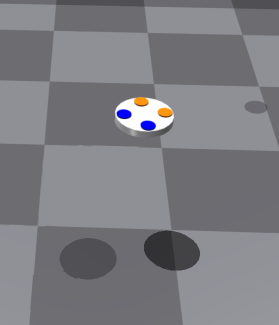
\includegraphics[width=\textwidth]{figures/6_/6_quadrotor.png}
         \caption{Quadrotor}
         \label{fig:6_quadrotor}
     \end{subfigure} 
     \hspace{0.15\textwidth}
     \begin{subfigure}[b]{0.32\textwidth}
         \centering
         \captionsetup{justification=centering}
         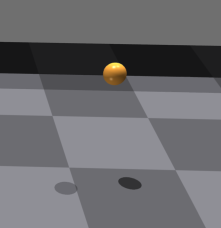
\includegraphics[width=\textwidth]{figures/6_/6_goal.png}
         \caption{Goal}
         \label{fig:6_goal}
     \end{subfigure} 
     \caption{Quadrotor and goal assets in our Isaac Gym environment. These are both standard assets already present in Isaac Gym, and are borrowed for this task. The quadrotor does not collide with the goal, nor is the goal visible in the depth images.}
     \label{fig:6_quad_goal}
\end{figure}

With defined collision geometries, we could then enable collisions in the environments by placing obstacles in the same environment in the same collision group and setting their collision filters to be 1. Since we do not want collisions with the goal, we removed its collision geometry, rendering it invisible to the depth camera and removing the possibility for collision. 

Finally, to place these obstacles nicely in our environment, we could change the object dimensions in the URDF files and do further scaling of objects in Isaac Gym. Then, through the root tensor, we adjusted their poses through rotations and randomised their position.

\begin{figure}[H]
     \centering
     \hspace{0.04\textwidth}
     \begin{subfigure}[b]{0.3\textwidth}
         \centering
         \captionsetup{justification=centering}
         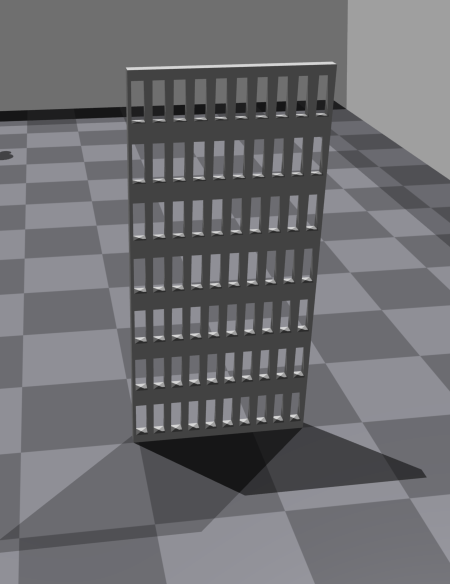
\includegraphics[width=\textwidth]{figures/6_/fence.png}
         \caption{Fence}
         \label{fig:6_obst_fence}
     \end{subfigure} 
     \hspace{0.15\textwidth}
     \begin{subfigure}[b]{0.3\textwidth}
         \centering
         \captionsetup{justification=centering}
         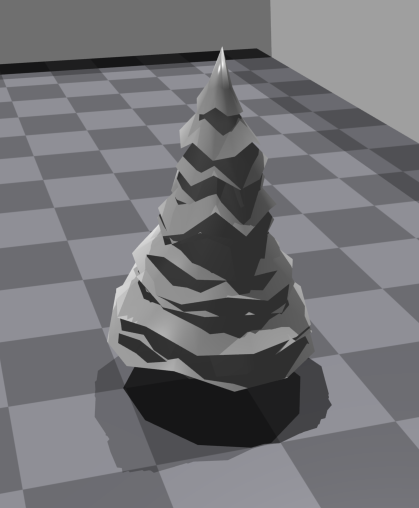
\includegraphics[width=\textwidth]{figures/6_/pine_tree.png}
         \caption{Pine tree}
         \label{fig:6_obst_pine_tree}
     \end{subfigure} 
     \hfill \\[2mm]
     \hspace{0.04\textwidth}
     \begin{subfigure}[b]{0.3\textwidth}
         \centering
         \captionsetup{justification=centering}
         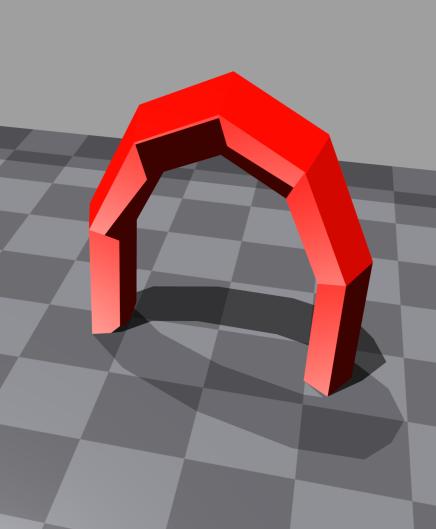
\includegraphics[width=\textwidth]{figures/6_/simple_u.png}
         \caption{Simple U-shape}
         \label{fig:6_obst_simple_u}
     \end{subfigure} 
     \hspace{0.15\textwidth}
     \begin{subfigure}[b]{0.3\textwidth}
         \centering
         \captionsetup{justification=centering}
         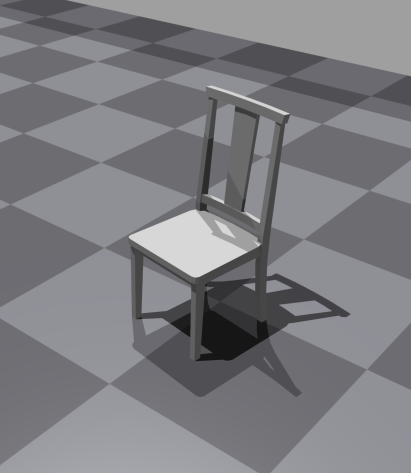
\includegraphics[width=\textwidth]{figures/6_/chair.png}
         \caption{Chair}
         \label{fig:6_obst_chair}
     \end{subfigure}
     \hfill \\[2mm]
     \hspace{0.04\textwidth}
     \begin{subfigure}[b]{0.3\textwidth}
         \centering
         \captionsetup{justification=centering}
         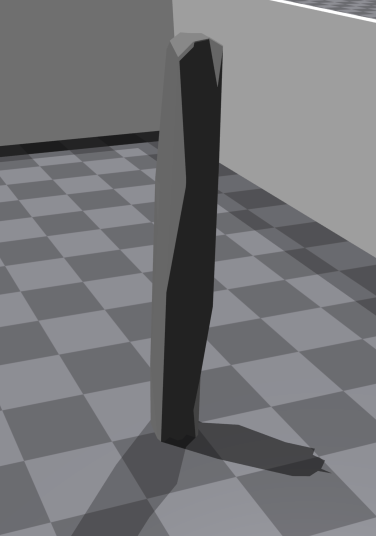
\includegraphics[width=\textwidth]{figures/6_/simple_stone.png}
         \caption{Simple stone}
         \label{fig:6_obst_simple_stone}
     \end{subfigure} 
     \hspace{0.15\textwidth}
     \begin{subfigure}[b]{0.3\textwidth}
         \centering
         \captionsetup{justification=centering}
         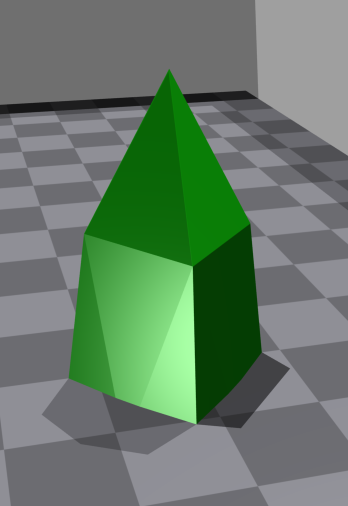
\includegraphics[width=\textwidth]{figures/6_/simple_pyramid.png}
         \caption{Simple pyramid}
         \label{fig:6_obst_simple_pyramid}
     \end{subfigure} 
    \caption{Various obstacles are imported to our Isaac Gym environment through their URDF files. Their defined collision geometries allows them to be visible in the depth images and allows the physics engine to simulate collisions with them. By altering their dimensions and \textit{root tensors}, we could fit them nicely in our environments, with randomised poses.}
     \label{fig:6_obstacles}
\end{figure}

\newpage
\subsection{Parallel Initialisation}
Regarding the parallel initialisation of the environments, this depends on which stage of the curriculum we are training on.
In the first scenario, with no obstacles, we initialise each environment to have a quadrotor and goal with random positions in an area $x, y \in [-3, 3]$, with $z \in [-0.2, 2]$. Furthermore, we add a ground plane at $z = 0$ and mimic ``far obstacles'' by confining each quadrotor to a $16\times8$ enclosure. This serves to bias the agent to initially ignore the depth representation input while it learns to map the quadrotor states to correct actions. 

Then, for 1-obstacle environments, the quadrotor and goal for each environment are now placed at each end of their enclosure, with an obstacle placed in the middle. Their initialised $x$ positions are fixed (along the long axis) but are randomised in $y$ (short axis). Also, the quadrotors and goals are slightly randomised in $z$. Then, we extend this design to $n$-obstacle environments, where we gradually increase the number of obstacles between a quadrotor and goal while ensuring that a quadrotor always has $3$m of open space before the first obstacle. An example is shown in \cref{fig:6_n_obst_env}.
\begin{figure}[hbt]
    \begin{subfigure}[b]{0.69\textwidth}
        \centering
        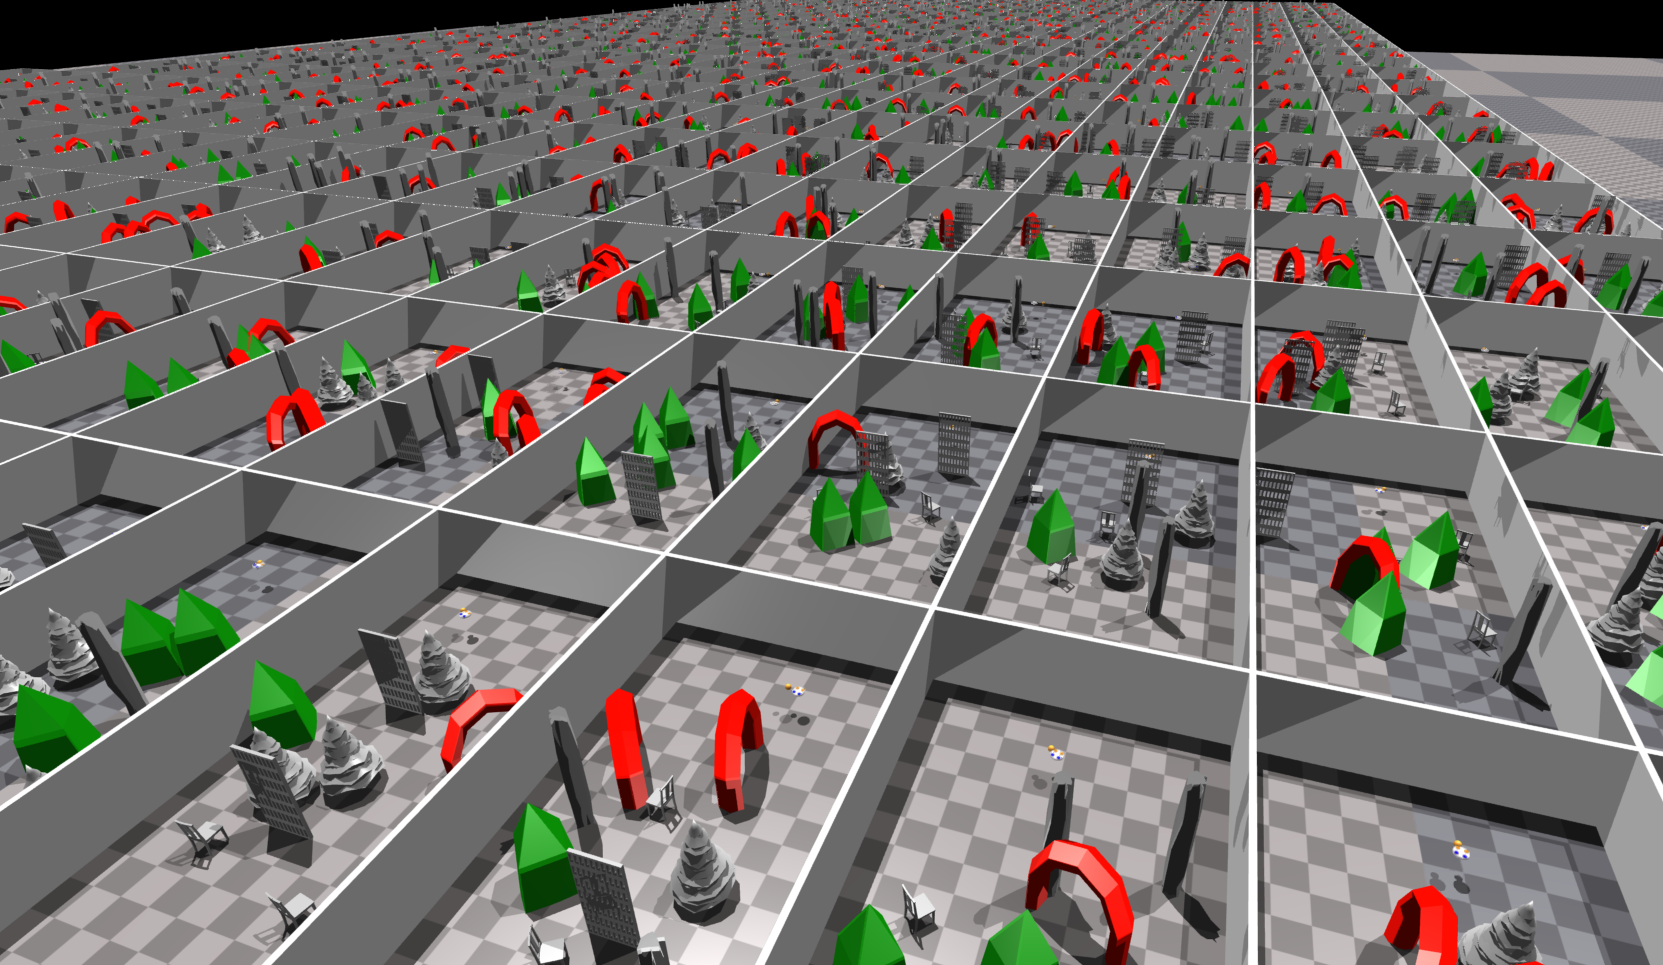
\includegraphics[width=0.99\textwidth]{figures/6_/6_environments.png}
        \caption{512 environments are initialisation in parallel, with randomised obstacles along $y$.\vspace{8mm}}
        \label{fig:6_environments}
    \end{subfigure}
    \hfill
    \begin{subfigure}[b]{0.3\textwidth}
        \centering
        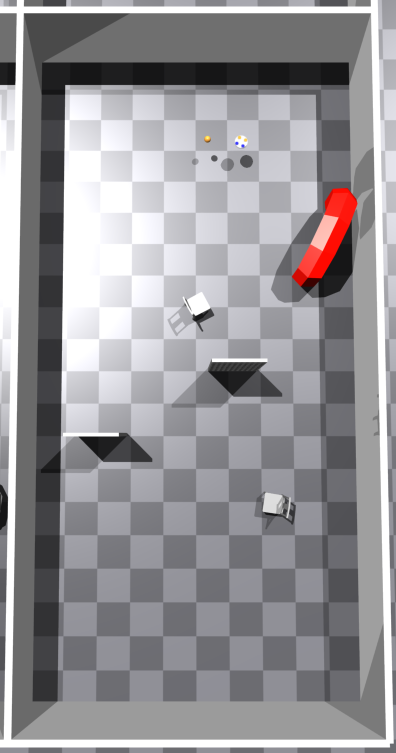
\includegraphics[width=0.7\textwidth]{figures/6_/6_n_obst_env.png}
        \caption{Quadrotor, goal and obstacle positions are randomised in $y$ for each environment.}
        \label{fig:6_n_obst_env}
    \end{subfigure}
    \caption{An example of the parallel initialisation of environments and their obstacle placements with Isaac Gym \cite{IsaacGym}. We simulate 512 environments in parallel, where the quadrotor and goal is initialised at each end of a corridor-like enclosure with obstacles placed in between. Positions of each item are fixed in the $x$ (long axis), but randomised in $y$ (short axis). Quadrotor and goal heights (in $z$) are also slightly randomised.}
    \label{fig:6_env_init}
\end{figure}


\section{Model Implementation and PPO in RL Games}
Now that the reinforcement learning framework was prepared, we used a reinforcement learning library called \textit{RL Games} \cite{rl-games2022} to implement our CNN-MLP network to be trained with PPO.
The RL Games integration with IsaacGym follows a strictly hierarchical structure where all specific algorithms and models inherit from general base implementations. In this way, the training setup is defined through configuration files managed by \textit{Hydra}\footnote{See how IsaacGymEnvs uses Hydra at \url{https://github.com/NVIDIA-Omniverse/IsaacGymEnvs}.}. 

\subsection{Implementing our Model}
\label{subsec:6_model_implementation}
To integrate our model with RL games, we identified that the main challenge is not how to implement PPO with our model but how to integrate our custom network into RL Games. If we could solve this, we could then specify that our model should use our custom network in configuration, and this should allow it to be seamlessly optimised with PPO.
So to solve this, we first wrapped our custom network in a \textit{network builder}. From here, we could use a \textit{model builder} to register our network in RL Games' network registry during initialisation. As a result, our network was now a part of RL games and could be chosen for any reinforcement learning task.

Then, to use it in our custom quadrotor task, we define two configuration files, one for the setup of the quadrotor task and the other to define the model. Here, the task configuration is quite standardised, including the dimension of observation and action space, simulation parameters like \textit{dt}, but also the number of obstacles, environment size and episode length. In contrast, the training file provided our model definition, consisting of the optimisation algorithm and its hyperparameters (batch size, learning rate, trajectory length, etc.), and our network and its hyperparameters (size, activation functions, normalised actions, separate actor-critic networks, etc.).

\subsection{Normalised and Clipped Observation and Action Space}
\label{subsec:6_normalisation}
Next, there are some noteworthy details of our model implementation that is relevant to our task. The first is that normalising the observation and action spaces is of particular importance in RL Games, first introduced in \cite{DDPG} and also iterated in the documentation of Stable-Baselines3, ``normalising input features may be essential to the successful training of an RL agent'' \cite{stable-baselines3}. \textit{Normalising} can mean two different things in reinforcement learning, either by scaling observations to $[0, 1]$ or to have 0 mean and 1 standard deviation. The perspective this thesis takes is that image values are scaled while everything else is normalised.
So, to normalise the observation space in our quadrotor task, RL Games keeps track of our running mean and standard deviation through its \textit{RunningMeanStd} class, which calculates its values throughout the training process. We also alter the code slightly to ensure that our depth images are not affected.
The consequence of this is that when we gradually increase the environment size to larger values, i.e. greater $\p_t$ from the goal, this should not alter the policy performance. 
For the actions, these are not normalised but instead clipped if their values exceed 1, which was also why we avoided using a non-linear activation function for our actor-critic. For good measure, the observations space is also clipped to a max value of 5 before being normalised, in case of, e.g. anomaly observations.

\subsection{Experience and Optimisation}
\label{subsec:6_experience_optimisation}
In order to perform optimisation, recall from \cref{subsec:2_PPO} that PPO requires data (experience) sampled by its current policy in a trajectory $\boldsymbol{T}$, where each \textit{experience} element is given by a tuple $<S_t, A_t, R_t, S_{t+1}$. In the parallel learning scheme, observations $S_t = [\s_t, \d_t]$ from each environment is compiled into an observation buffer $\boldsymbol{O}_t$ for each time timestep. As mentioned, these observations are then clipped and normalised before being sent to the actor to provide actions for the current policy $\pi$. Though we simulate 512 environments, there is only one network -- for each timestep, we batch the 512 observations into an input tensor of shape $[512, 129613]$ and compute the forward-pass for the whole batch. The batched depth images are sent separately to the VAE, which produces the latent code with dimension $[512, 64]$. Then, by concatenating it with the quadrotor state tensor to get $[512, 64]$, our actor-critic outputs a batched action tensor of shape $[512, 3]$. Finally, our agent observes rewards $R_t$ with dimension $[512, 1]$ to which it can compare to its value estimates $V_t$ to calculate the advantage estimate $\hat{A}_t$.

Throughout this process, an \textit{experience buffer} collects the state-action pairs as the trajectory. We define the \textit{horizon} or size of the \textit{trajectory} $\boldsymbol{T}$ to be $8$, such that our batch size is $512\cdot8 = 4096$. We also define a minibatch size of $M=1024$ and a number of mini-epochs $K=8$. Overall, we first simulate our environment in parallel for 8 timesteps to collect a trajectory. With this, we optimise for our PPO loss in mini-batches and repeat the optimisation on the trajectory for $K=8$ mini-epochs. Finally, we discard the trajectory and run the simulation for 8 timesteps to collect a new trajectory and so on. Lastly, when calculating the gradients for the trajectory, we also utilise truncated gradients where the gradients are scaled according to Pytorch's \textit{GradScaler} and clipped by their norm. These gradients are then used to optimise our network weights through the \textit{Adam} optimiser \cite{adam}.

\subsection{Reset Handling}
\label{subsec:6_reset_handling}
When calculating gradient updates, the PPO critic value is used to calculate the advantage $\widehat{A}_t = Q(s,a) - V_{\bt}(s)$, where $V_{\bt}(s)$ is the predicted infinite sum of discounted rewards (predicted return). In our experiments, we specify a max episode length $T$ that resets environments at this timestep. However, from what is seen in the experience buffer, resets count as a state-``transition'' for which the action performed suddenly leads to a drastic change in reward.
Since these resets cannot be predicted, this can lead to inferior critic updates as the prediction error in \eqref{eq:2_ppo_critic_loss} for these resets are severely incorrect. To handle this, the target of the critic is bootstrapped with its own prediction during resets, such that the critic error is only the reward obtained for the first timestep in the next episode.